\documentclass[../sections/subsections/probabilidad_condicional.tex]{sufiles}

% Set the overall layout of the tree
\tikzstyle{level 1}=[level distance=3.5cm, sibling distance=3.5cm]
\tikzstyle{level 2}=[level distance=3.5cm, sibling distance=2cm]

% Define styles for bags and leafs
\tikzstyle{bag} = [text width=4em, text centered]
\tikzstyle{end} = [circle, minimum width=3pt,fill, inner sep=0pt]

% The sloped option gives rotated edge labels. Personally
% I find sloped labels a bit difficult to read. Remove the sloped options
% to get horizontal labels. 
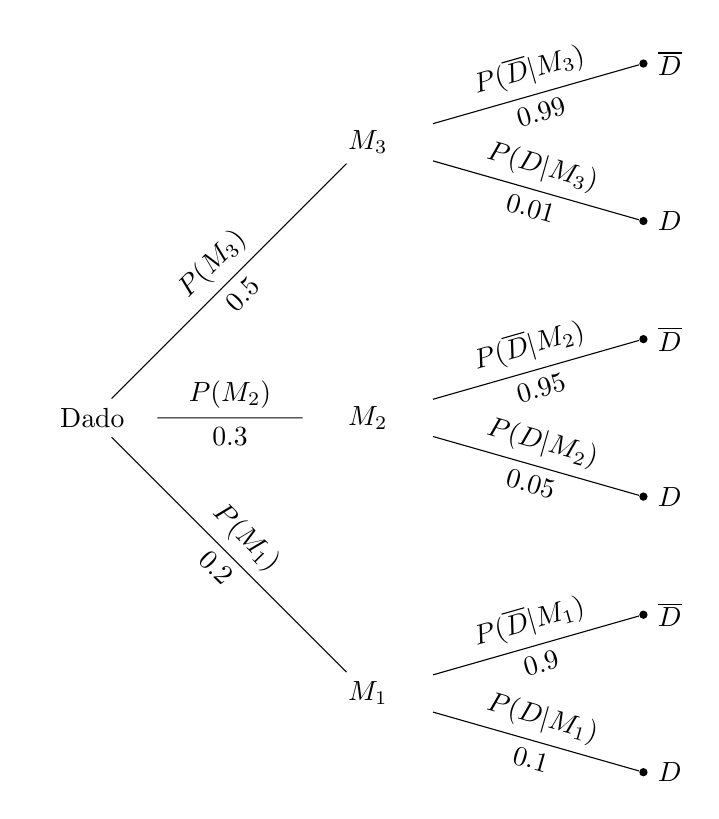
\begin{tikzpicture}[grow=right, sloped]
\node[bag] {Dado}
    child {
        node[bag] {$M_{1}$}        
            child {
                node[end, label=right:
                    {$D$}] {}
                edge from parent
                node[above] {$P(D|M_{1})$}
                node[below]  {$0.1$}
            }
            child {
                node[end, label=right:
                    {$\overline{D}$}] {}
                edge from parent
                node[above] {$P(\overline{D}|M_{1})$}
                node[below]  {$0.9$}
            }
            edge from parent 
            node[above] {$P(M_{1})$}
            node[below]  {$0.2$}
    }
    child {
        node[bag] {$M_{2}$}        
            child {
                node[end, label=right:
                    {$D$}] {}
                edge from parent
                node[above] {$P(D|M_{2})$}
                node[below]  {$0.05$}
            }
            child {
                node[end, label=right:
                    {$\overline{D}$}] {}
                edge from parent
                node[above] {$P(\overline{D}|M_{2})$}
                node[below]  {$0.95$}
            }
            edge from parent 
            node[above] {$P(M_{2})$}
            node[below]  {$0.3$}
    }
    child {
        node[bag] {$M_{3}$}        
            child {
                    node[end, label=right:
                        {$D$}] {}
                    edge from parent
                    node[above] {$P(D|M_{3})$}
                    node[below]  {$0.01$}
                }
            child {
                node[end, label=right:
                    {$\overline{D}$}] {}
                edge from parent
                node[above] {$P(\overline{D}|M_{3})$}
                node[below]  {$0.99$}
            }
        edge from parent         
            node[above] {$P(M_{3})$}
            node[below]  {$0.5$}
    };
\end{tikzpicture}